\chapter{Experimentos}\label{chapter:implementation}
En este capítulo se presentan una serie de experimentos diseñados para evaluar el rendimiento y las capacidades del agente \textit{lImporter}. Es importante aclarar que no se realizó un análisis holístico y cuantitativo del sistema. En su lugar, se optó por explorar distintos casos de uso que demuestran la versatilidad de la herramienta y ponen de manifiesto las interesantes posibilidades que surgen al integrar un agente de lenguaje autónomo en una bóveda de conocimiento de \textit{Obsidian}.

\section{Base estructurada sobre \textit{Harry Potter}}
En el primer experimento, se utilizó la versatilidad del agente para una tarea clásica: la creación de una base de conocimientos estructurada sobre el universo de \textit{Harry Potter}. El objetivo era proporcionar al agente el \textit{PDF} del primer libro y pedirle que generara notas para personajes, lugares y conceptos clave, vinculándolos entre sí. El agente generó exitosamente un total de 296 notas (entidades) y 671 enlaces entre ellas. Este caso de uso potencia a \textit{Obsidian} como una herramienta para la exploración visual del conocimiento a través de su vista de grafo.

Es relevante mencionar que, por defecto, \textit{Obsidian} no muestra etiquetas en las aristas del grafo, lo que dificulta la interpretación de la naturaleza de las relaciones. Para solventar esto, se utilizó un \textit{plugin} llamado \textit{Graph Link Types} de la comunidad que añade dicha funcionalidad. El grafo resultante, como se muestra en la Figura \ref{fig:hp_graph}, fue creado exitosamente. 

\begin{figure}[h]
    \centering
    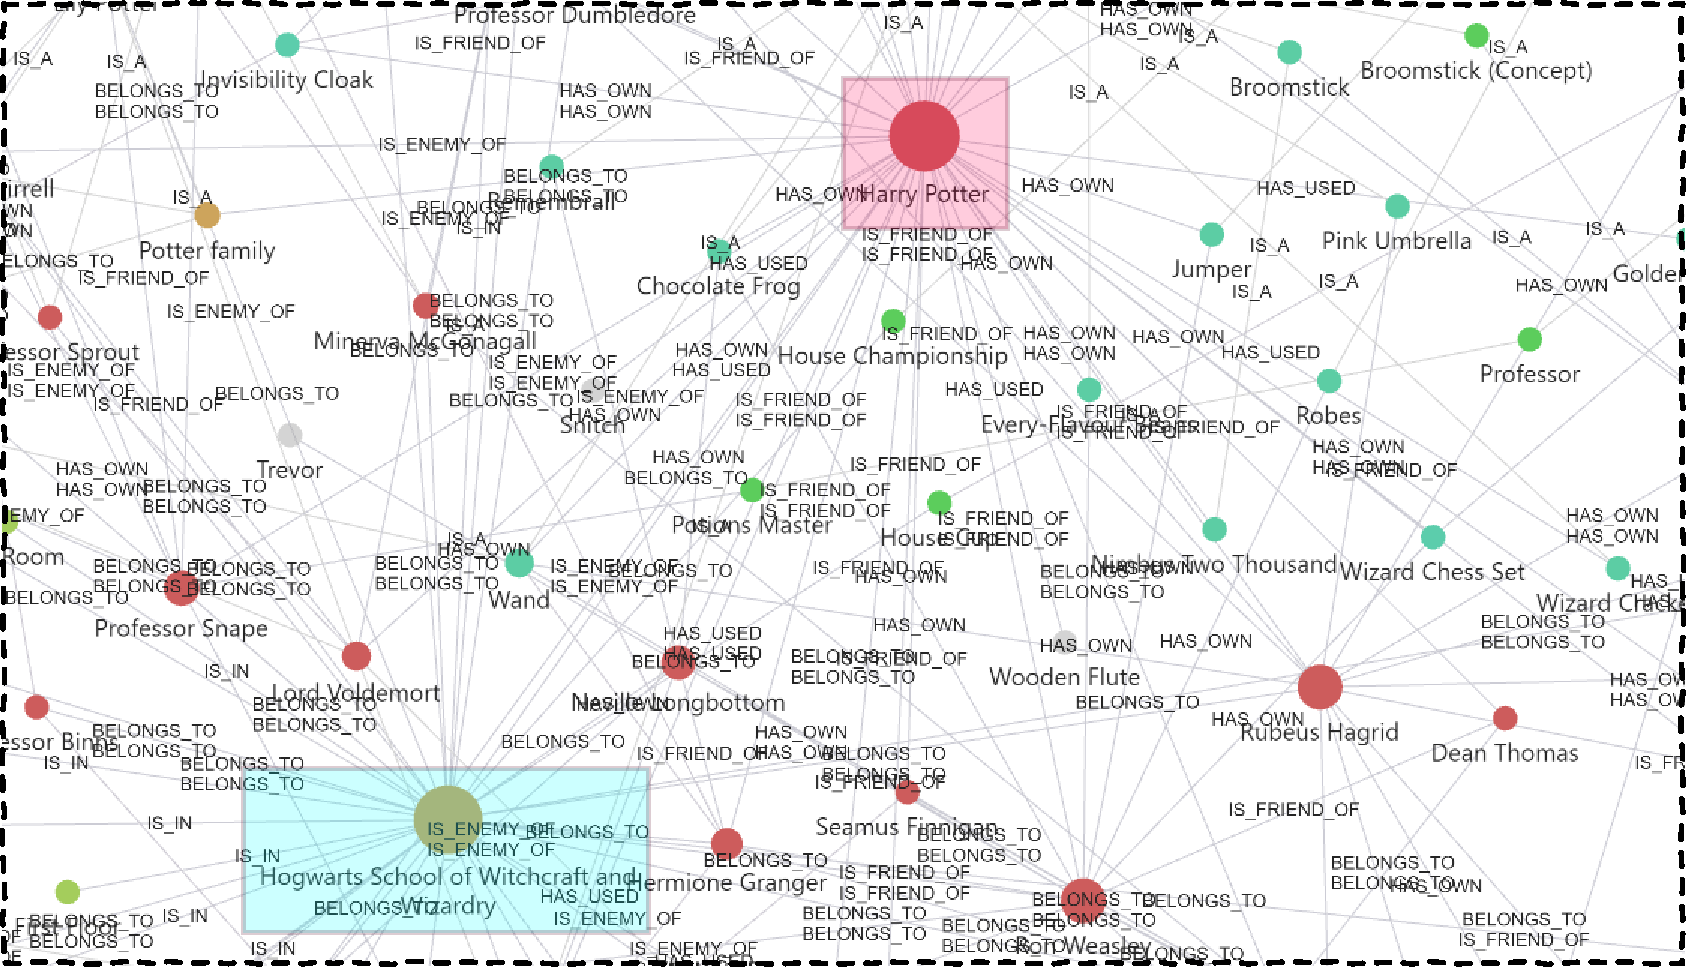
\includegraphics[width=1.0\textwidth]{figures/HPKG.pdf}
    % \fbox{\parbox[c][15em][c]{0.8\textwidth}{\centering \huge Placeholder: \\ Grafo de conocimiento de Harry Potter generado por el agente}}
    \caption{Grafo resultante del experimento de \textit{Harry Potter}, mostrando la centralidad de nodos clave.}
    \label{fig:hp_graph}
\note{En la figura, se observa que conceptos centrales como \textit{Harry Potter} (resaltado en rojo) y \textit{Hogwarts} (en azul) se representan con nodos de mayor tamaño. Esto se debe a que \textit{Obsidian} modula el tamaño de cada nodo en función de su grado —el número de conexiones que posee—, lo que resalta visualmente la importancia de las entidades más conectadas y demuestra la utilidad de esta representación incluso para bases de conocimiento ya estructuradas.}
\end{figure}

Es importante señalar que este experimento no fue diseñado con el objetivo de realizar una extracción de entidades exhaustiva y precisa. Su propósito principal era demostrar la capacidad del sistema para abordar un caso de uso estructurado con la configuración adecuada. Aun así, los resultados evidencian cómo el agente puede generar rápidamente una representación del conocimiento que es tanto visualmente atractiva como funcional, constituyendo un excelente punto de partida para el análisis preliminar de cualquier dominio.

\section{Añadiendo artículos a una \textit{Wiki} tecnológica}
Este experimento se diseñó para simular el mantenimiento y crecimiento de una base de conocimiento existente. Se partió de una bóveda de \textit{Obsidian} que funcionaba como una \textit{wiki} personal sobre temas de tecnología (programación, \textit{hardware/software}, etc.). Progresivamente, se le proporcionaron al agente nuevos archivos, acompañados de un breve audio con instrucciones.

\begin{figure}[h!]
    \centering
    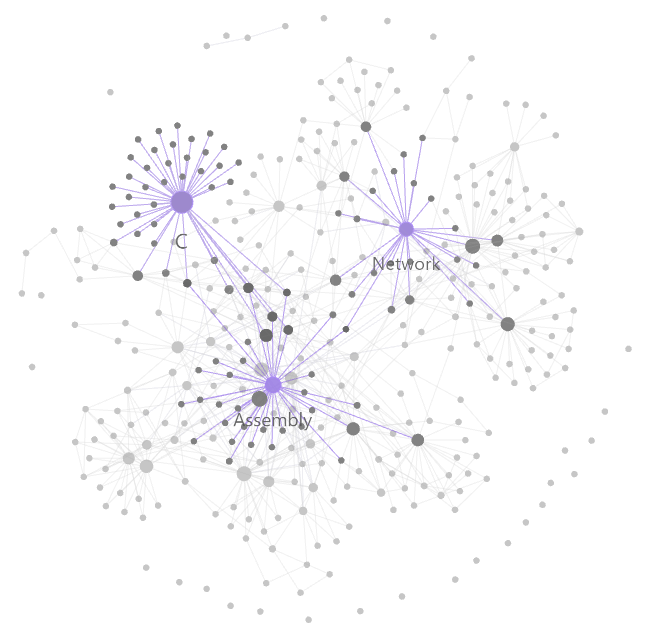
\includegraphics[width=0.6\textwidth]{figures/WikiSamples2.png}
    \caption{\textit{Wiki} personal sobre temas de tecnología.}
    \label{fig:wiki_tech_graph}
\end{figure}

El objetivo era doble. Por un lado, se buscaba demostrar que el agente es capaz de analizar el nuevo contenido, comprenderlo en el contexto de la bóveda existente y determinar correctamente con qué notas preexistentes debía vincularlo. Por otro lado, y de igual importancia, se quería verificar que el agente no siempre establece conexiones. Si un nuevo artículo trata sobre un tema completamente ajeno a lo que ya existe en la bóveda, el resultado deseable es que se cree una nota aislada, sin vínculos forzados o incorrectos. Este comportamiento es crucial para mantener la integridad y la calidad del grafo de conocimiento.

Para evaluar estos comportamientos, se realizaron dos secuencias de inserción. En la primera, se introdujeron artículos sobre \textit{hardware} neuromórfico y alternativas a \textit{backpropagation}, temas sin representación previa en la bóveda. Como se esperaba, el agente creó las notas correspondientes (visibles en su totalidad en la Figura \ref{fig:wiki_isolated}) pero no las vinculó con el grafo existente. En la segunda secuencia, se añadió una serie de artículos sobre los orígenes de las \textit{Interaction Nets} y sus aplicaciones actuales. En este caso, el agente creó las siguientes notas, vinculándolas a 7 notas preexistentes:
\begin{itemize}
    \item \textit{Interaction Nets.md}
    \item \textit{Interaction Combinators.md}
    \item \textit{HVM2.md}
    \item \textit{Bend.md}
\end{itemize}
El resultado de esta integración se muestra parcialmente en la Figura \ref{fig:wiki_connected}, donde se aprecian las nuevas notas conectadas al conocimiento previo.

\begin{figure}[h!]
    \centering
    \begin{subfigure}[b]{0.48\textwidth}
        \centering
        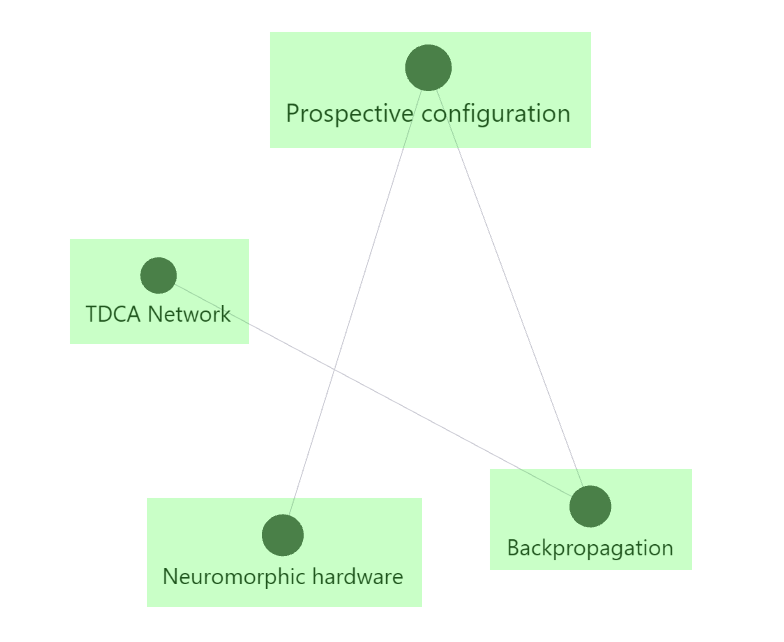
\includegraphics[width=\textwidth]{figures/neuromPart.png}
        % \fbox{\parbox[c][12em][c]{0.9\textwidth}{\centering \huge Placeholder: \\ Grafo de nodo aislado}}
        \caption{Notas sobre \textit{hardware} neuromórfico sin conexiones externas a las nuevas.}
        \label{fig:wiki_isolated}
    \end{subfigure}
    \hfill
    \begin{subfigure}[b]{0.5\textwidth}
        \centering
        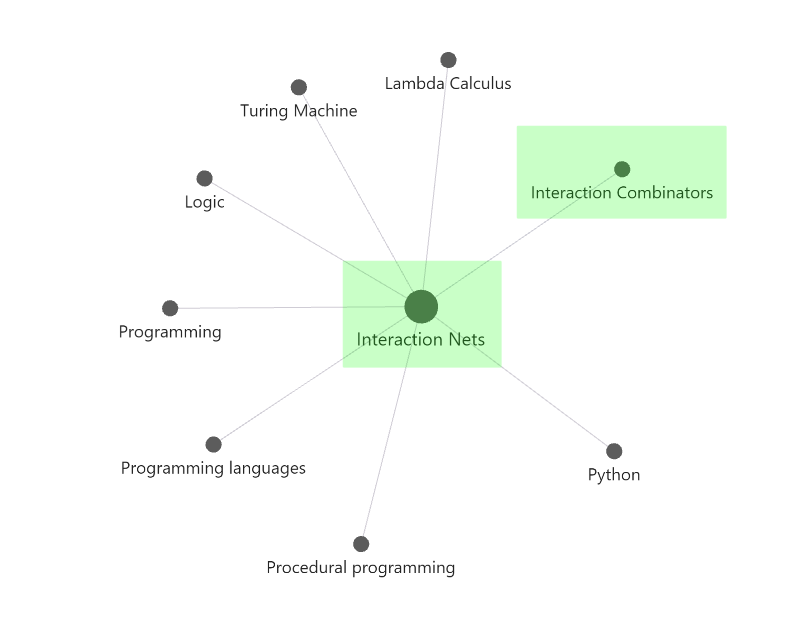
\includegraphics[width=\textwidth]{figures/IntNetsPart.png}
        % \fbox{\parbox[c][12em][c]{0.9\textwidth}{\centering \huge Placeholder: \\ Grafo local conectado}}
        \caption{Notas sobre \textit{Interaction Nets} conectadas a notas existentes.}
        \label{fig:wiki_connected}
    \end{subfigure}
    \caption{Comparación de resultados de inserción con las notas nuevas resaltadas.}
    \label{fig:wiki_comparison}
\note{Ambas vistas corresponden al grafo local de \textit{Obsidian}. En el caso aislado (izquierda), se muestra con profundidad máxima (5), pero al no tener vínculos, solo aparecen los nodos resultantes de la secuencia de inserción. En el caso conectado (derecha), una profundidad de 1 es suficiente para visualizar las conexiones a notas existentes.}
\end{figure}

En conjunto, estos resultados verifican la versatilidad del agente para determinar, de forma autónoma, qué notas existentes son candidatas idóneas para establecer vínculos con el nuevo contenido. Esta capacidad de discernimiento, reforzada por el optimizador de contexto, es fundamental para asegurar que la base de conocimiento crezca de manera coherente y relevante.

\section{\textit{Projects, Areas, Resources, Archived}}
Este experimento refleja un caso de uso más cotidiano y de productividad personal, siguiendo la metodología \textit{P.A.R.A}. \textit{(Projects, Areas, Resources, Archived)} popularizada por \cite{forteBuildingSecondBrain2022}. El objetivo era evaluar si el sistema puede ser utilizado para mantener una bóveda organizada bajo esta estructura, siguiendo instrucciones de voz. Para ello, se realizaron 4 peticiones donde cada una consistía en un archivo de audio, acompañado opcionalmente por archivos de contexto adicionales.

Se evaluó la capacidad del modelo para realizar diversas tareas, entre las que destacan:
\begin{itemize}
    \item \textbf{Agregar detalles a proyectos existentes:} Por ejemplo, se solicitó añadir una nueva canción al proyecto de práctica de canto, proporcionando como contexto un documento con la letra adicional al audio con la instrucción.
    \item \textbf{Reescribir y sintetizar información:} Se instruyó por voz al modelo para que buscara información dispersa sobre un proyecto de tesis dentro de la bóveda. El contenido encontrado fue sintetizado en un nuevo documento. Además se propusieron nuevas ideas para complementar el trabajo en un documento adicional.
    \item \textbf{Crear nuevos proyectos:} Se crearon proyectos desde cero con indicaciones sobre sus objetivos y se vincularon a otros existentes. Por ejemplo, se generó un 'Nuevo proyecto de proyección vocal' vinculado al proyecto de 'práctica de canto'.
\end{itemize}

Como resultado de estas 4 peticiones, se crearon un total de 6 notas nuevas, sin incluir los archivos de transcripción. La Figura \ref{fig:para_synthesis} muestra un ejemplo de una de estas notas generadas, donde se sintetiza información dispersa y se vincula con otros proyectos.

\begin{figure}[h!]
    \centering
    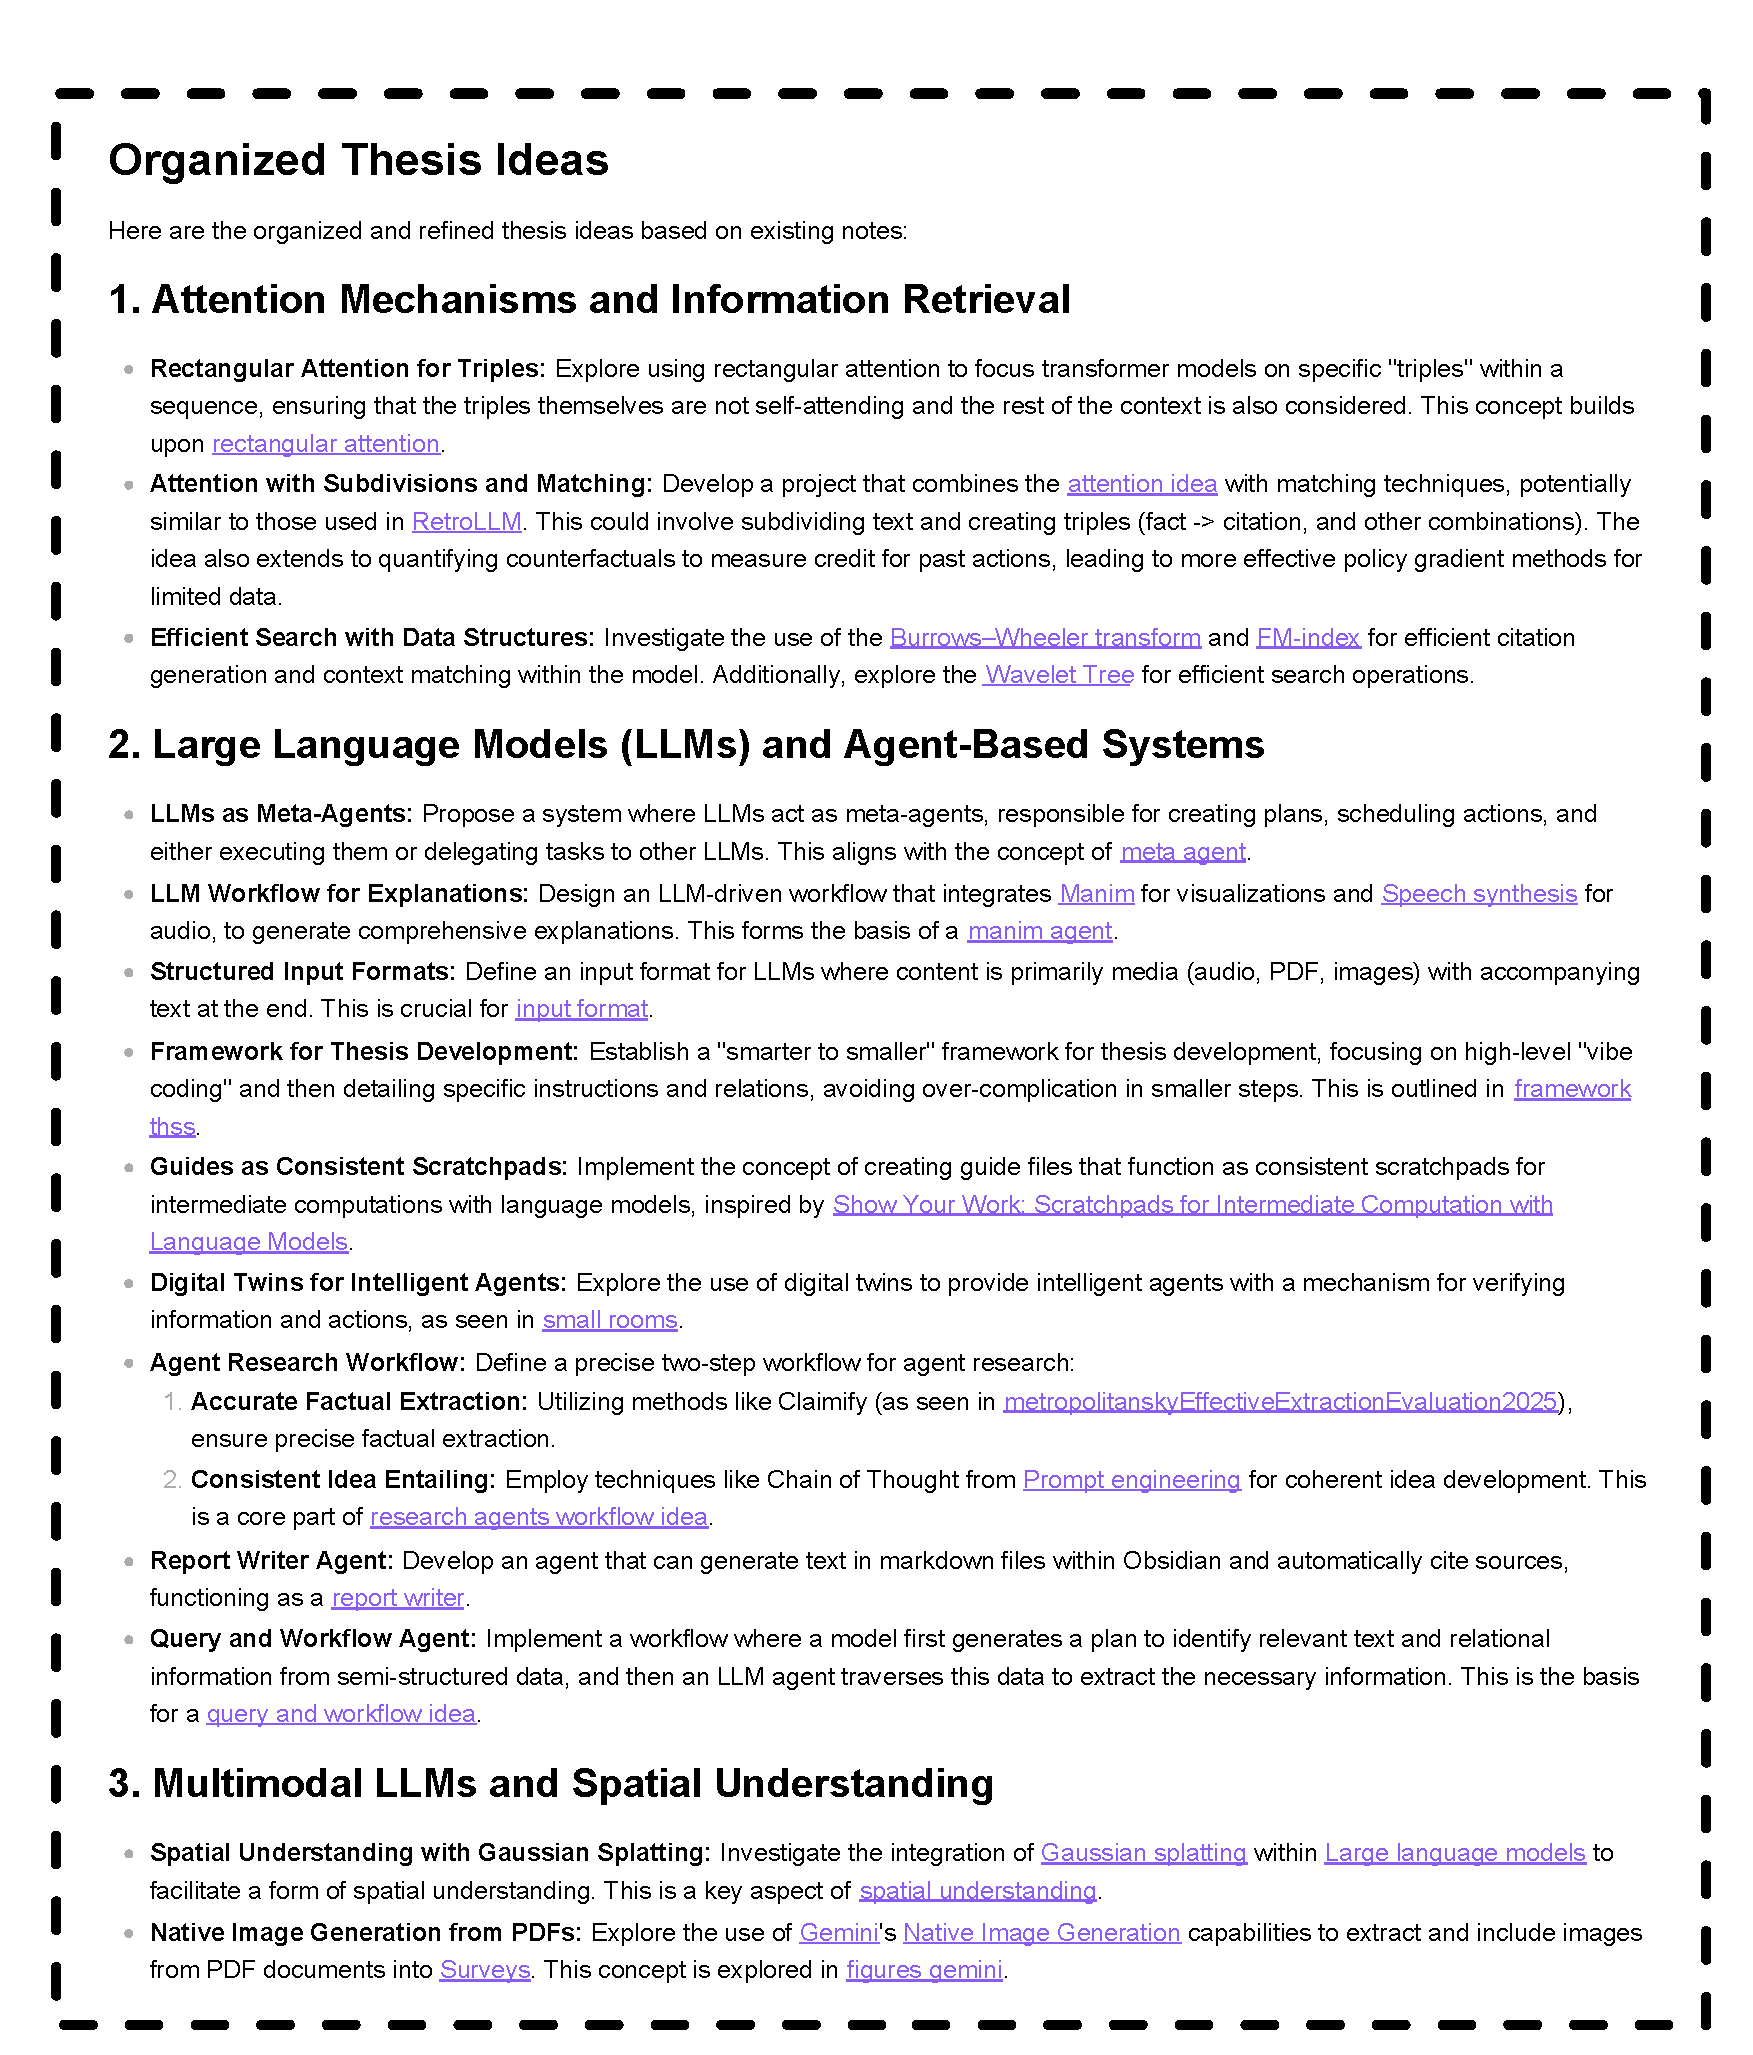
\includegraphics[width=0.8\textwidth]{figures/ideaSynthBx.pdf} 
    % \fbox{\parbox[c][12em][c]{0.8\textwidth}{\centering \huge Placeholder: \\ Ejemplo de nota de síntesis P.A.R.A.}}
    \caption{Ejemplo de una nota generada por el agente. Se sintetiza información sobre un proyecto de tesis y se enlaza a notas existentes.}
    \label{fig:para_synthesis}
\end{figure}

Adicionalmente, este experimento contaba con instrucciones para la automatización de flujos. El agente no solo procesaba la petición, sino que también movía automáticamente el archivo de audio a una carpeta designada y generaba un archivo de transcripción en la misma ubicación, organizando así los ficheros procesados y probando sus capacidades para automatizar tareas. Incluir los archivos generados en este documento sería verboso y no aportaría más información que la confirmación de que fueron creados correctamente. Por ello, los resultados y los nuevos ficheros se pueden consultar en el repositorio del proyecto.

\section{\textit{Note augmented LLMs are computationally universal}}
Este último experimento, de naturaleza más teórica, se inspira en la idea de que los modelos de lenguaje, cuando se aumentan con una memoria externa, pueden volverse computacionalmente universales \parencite{schuurmansMemoryAugmentedLarge2023}.

Para explorar esta idea, se le pidió al agente que evaluara la Conjetura de Collatz para un número dado, utilizando una nota de \textit{Obsidian} como su \textit{memoria de trabajo} o registro. En cada paso de la secuencia, el agente leía el estado actual de la nota, calculaba el siguiente número, y sobrescribía la nota con el nuevo valor.

\begin{figure}[h]
    \centering
    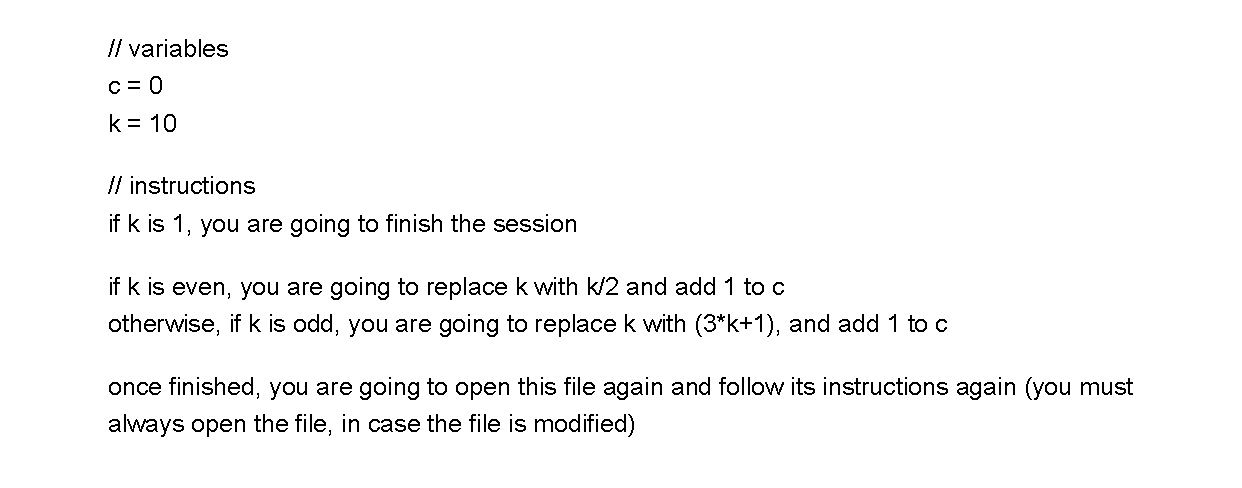
\includegraphics[width=1.0\textwidth]{figures/collatz_init_10.pdf}
    % \fbox{\parbox[c][15em][c]{0.45\textwidth}{\centering \huge Placeholder: \\ Contenido de la nota de Collatz}}
    \caption{Contenido inicial de la nota de trabajo para $n=10$ en la evaluación de Collatz.}
    \label{fig:collatz_code}
\end{figure}

Se evaluó el caso para $n=10$, que se resolvió correctamente en 6 iteraciones (Figuras \ref{fig:collatz_code} y \ref{fig:collatz_diff}). También se evaluaron casos más largos como $n=11$ (14 iteraciones) y $n=27$ (111 iteraciones). Este último caso excedió los límites de cuota de la \textit{API} y requirió reiniciar el proceso, lo cual demostró una capacidad emergente del sistema: la posibilidad de dejar una tarea y seguirla luego, ya que el estado se preserva en la nota de \textit{Obsidian}.

La intuición subyacente es que la capacidad de releer el estado desde un archivo fiable reduce drásticamente la probabilidad de error en un proceso iterativo largo, de manera análoga a cómo una \textit{CPU} depende de leer y escribir correctamente en sus registros. En este caso se usó un modelo potente en razonamiento algebraico (\textit{Gemini 2.5 Flash}). Si bien un modelo más modesto podría fallar en esta tarea matemática, la misma arquitectura podría permitirle automatizar con alta fiabilidad otra tarea iterativa que se alinee con sus fortalezas (por ejemplo, un análisis de sentimiento refinado a lo largo de múltiples revisiones), siempre que sea proficiente en las operaciones básicas de leer y escribir en su memoria externa.

\begin{figure}[h]
    \centering
    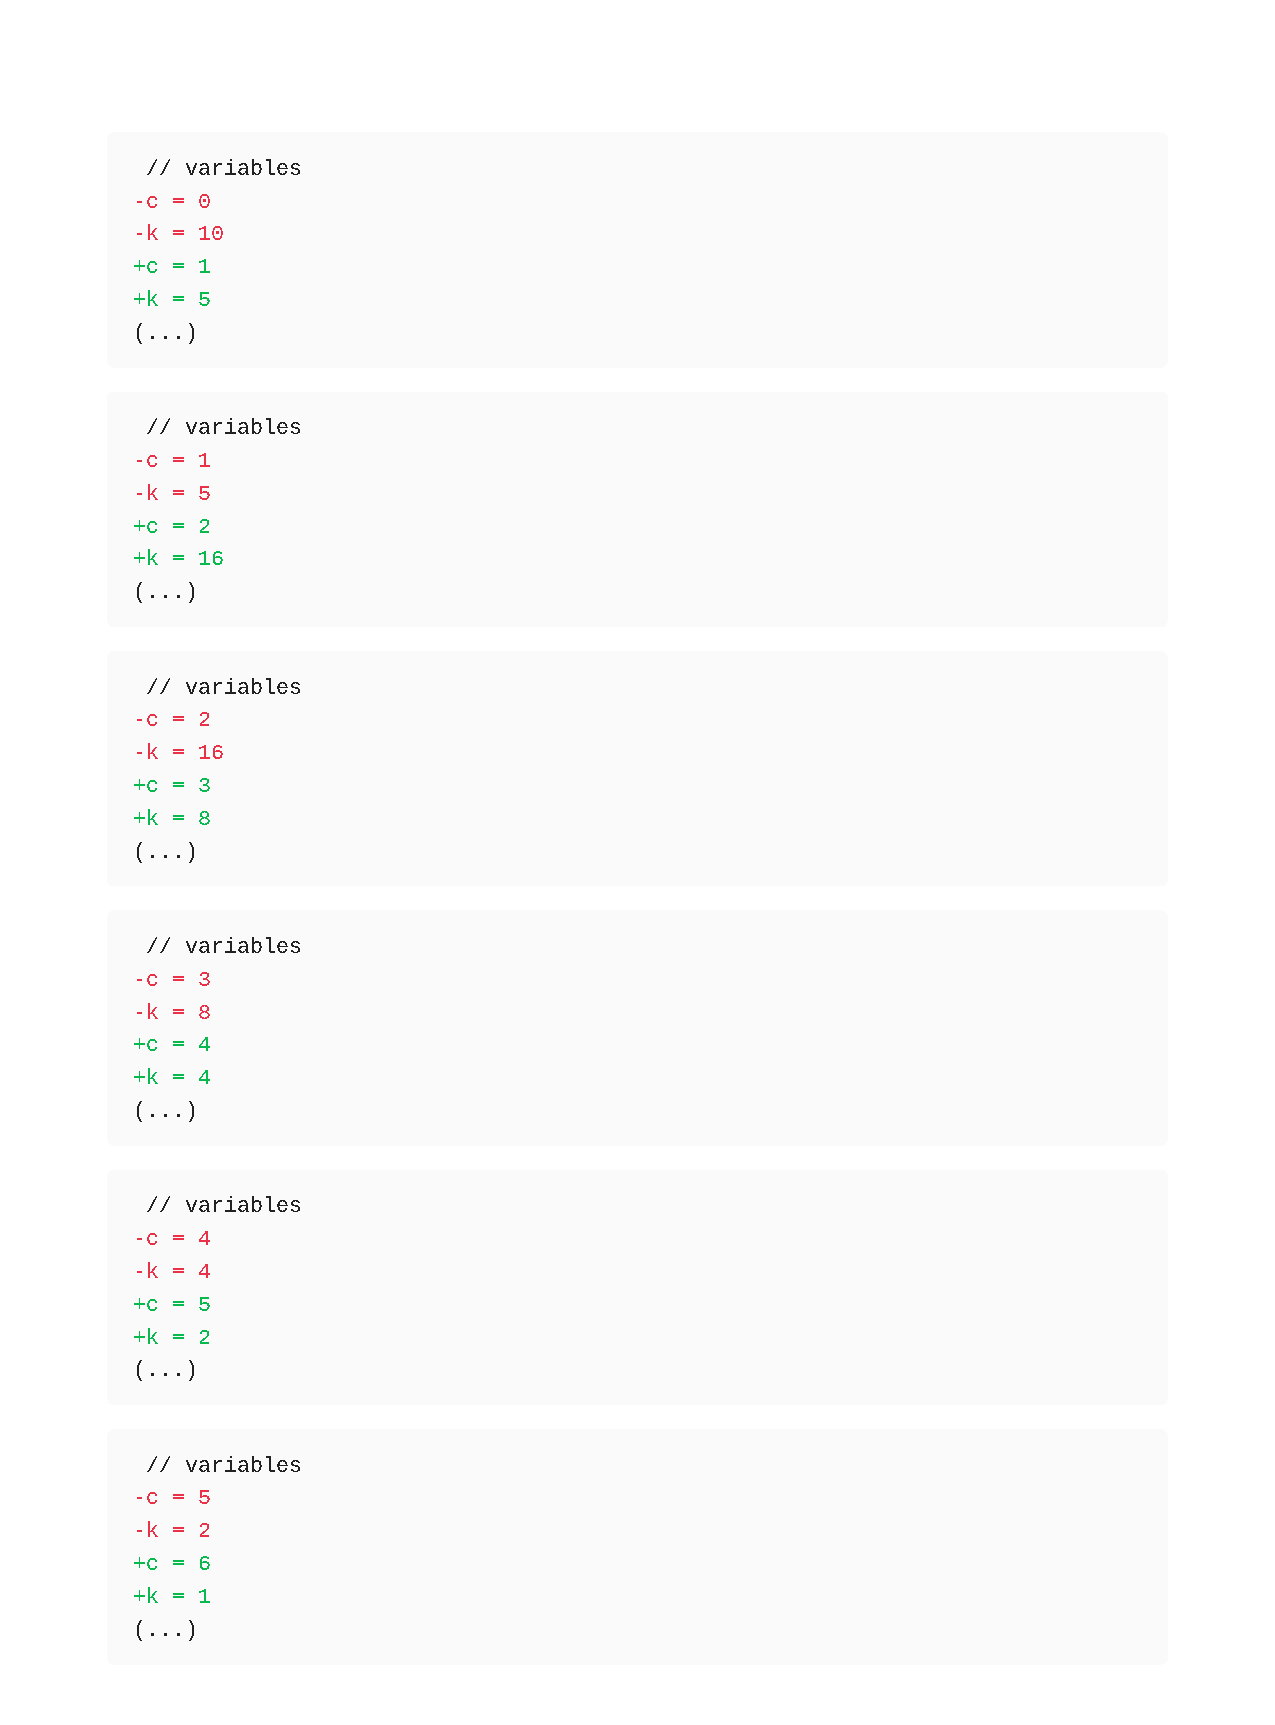
\includegraphics[width=1.0\textwidth]{figures/clltz_logs_10.pdf}
    % \fbox{\parbox[c][15em][c]{0.45\textwidth}{\centering \huge Placeholder: \\ Diff entre iteraciones}}
    \caption{Diferencia en el contenido de la nota entre los pasos de la evaluación para $n=10$.}
    \label{fig:collatz_diff}
\end{figure}